\documentclass[12pt]{article}
\usepackage{fullpage,graphicx,psfrag,amsmath,amsfonts,verbatim}
\usepackage{hyperref}
\usepackage[small,bf]{caption}

\input defs.tex

\bibliographystyle{alpha}

\title{
Estimating the Discrete Fourier Transform using Deep Learning
}

\author{
  Jonathan~Tuck\\
  Department of Electrical Engineering\\
  Stanford University\\
  \texttt{jtuck1@stanford.edu} \\
}
\begin{document}
\maketitle

\begin{abstract}
Throughout a wide variety of fields, the Discrete Fourier Transform (DFT) is used as a method of analysis 
of a signal's frequency components. In this paper, we show that a simple three-layer neural network with linear activation 
functions can estimate the DFT to high accuracy. We test our architecture on a variety of signals, and gauge both its 
accuracy and its speed against the ground truth and its fast, state-of-the-art implementation. We find that our neural 
network architecture achieves results very close to that of the ground truth, and that our implementation for our problem 
instance provides extremely similar accuracy, and is faster than both the naive implementation and the 
state-of-the-art implementation.
\end{abstract}

\section{Introduction}
Throughout a wide variety of fields -- from signal processing \cite{OS:99}, to medical imaging \cite{S:00}, 
to optics \cite{G:96} -- the Fourier Transform has been used as an important tool for signal analysis, allowing 
one to decompose a signal in space or time into its frequency components. Typically, when one wants to analyze a 
signal, it requires the knowledge of the Fourier Transform (sometimes referred to as the \emph{spectrum}) of the 
signal. 
% Unfortunately, unknown signals' spectrums are typically only found by computing their Fourier transform 
% and manually inspecting any important attributes, which is typically both computationally expensive and laborious.

% Currently, the method of computing a Fourier transform for a discrete-time signal in $\reals^N$, the Discrete 
% Fourier Transform (DFT), can be computed in $O(N^2)$ time. However, there exists a fast and efficient 
% method of computing the DFT, the Fast Fourier Transform (FFT), which can be computed 
% in $O(N \log N)$ time \cite{B:78,O:17}.

The goal of this project is to estimate the DFT of a signal using a neural network architecture.
This neural network should be able to estimate the Discrete Fourier Transform of the signal without 
having to explicitly compute the Discrete Fourier Transform. Ultimately, the results of this project may lead to 
a robust deep learning architecture able to compute the DFT of a signal faster than the current state-of-the-art 
algorithm, the FFT \cite{CT:65}.

\section{The Discrete Fourier Transform}
The context and background for this project is abundant. Although there exist many formulations of the Fourier 
transform \cite{O:17}, the scope of this project will only deal with the (real part of the) DFT, the version that maps from 
discrete-time to discrete-time, as that is what computers mathematically can handle. The \emph{$N$-point DFT} 
$F: \reals^N \rightarrow \reals^N$ for an $N$-dimensional discrete-time signal \cite{B:78,O:17} 
$f = (f[0], f[1], \ldots, f[N-1])$ is defined as
\BEQ \label{e-DFT}
F\{f\}[m] = \sum_{n=0}^{N-1} f[n] e^{2 \pi i m n / N}, \quad m = 0, \ldots, N-1.
\EEQ
Figure \ref{f-example_DFT} illustrates a simple example of a discrete-time signal $f[n]$ and the real part 
of its DFT, Re$\{F\{f\}[m]\}$.

\begin{figure}
\centering
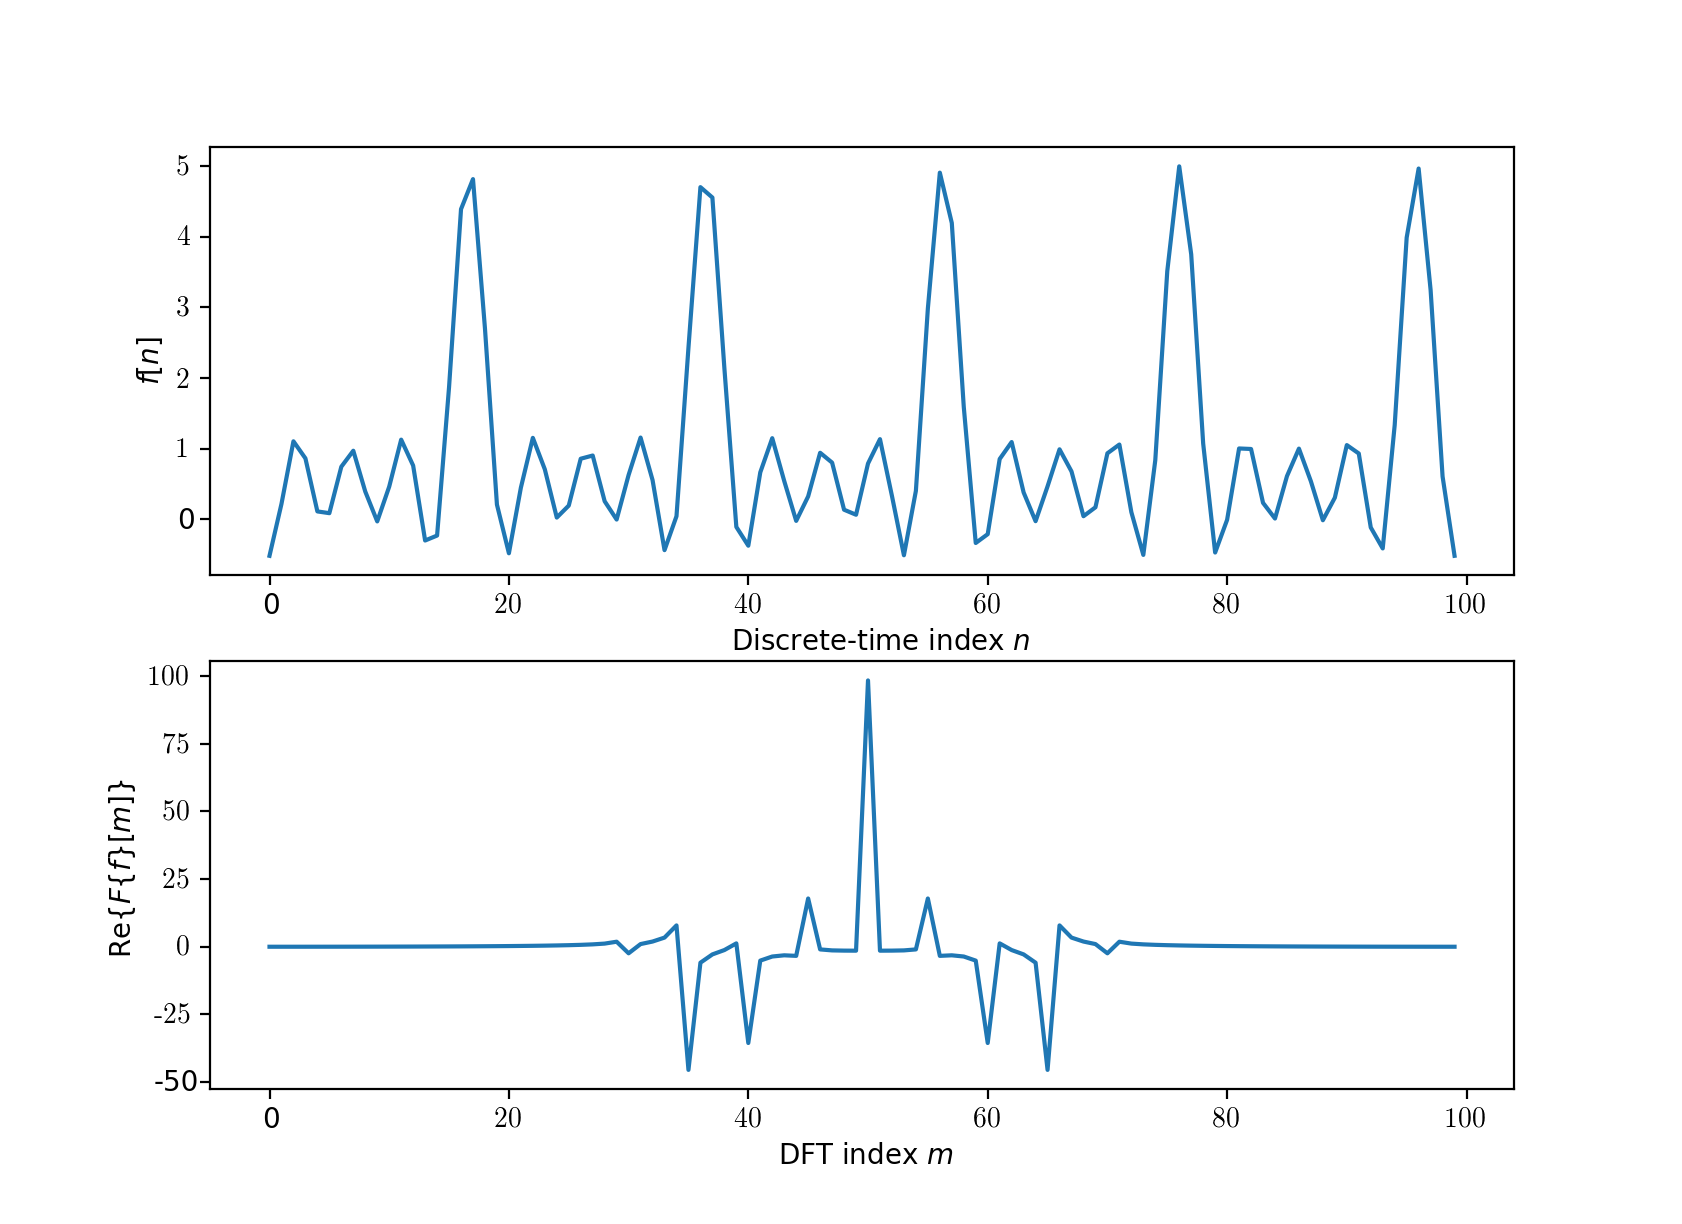
\includegraphics[scale=.5]{figures/DFT_example.png}
\caption{Discrete-time signal $f[n] = \sum_{i=1}^5 \cos(2 \pi i n + i)$ and 
the real part of its DFT, Re$\{F\{f\}[m]\}$.}
\label{f-example_DFT}
\end{figure}

The DFT in equation~(\ref{e-DFT}) can be written as a dense (complex-valued) matrix multiplication, \ie,
$F\{f\} = D f,$ where $D \in \complexs^{N \times N}$ is a complex matrix with values $e^{2 \pi i m n / N}$ in 
the $(m,n)$-index. As the DFT can be computed via a dense matrix multiplication, one can compute the DFT naively
in $O(N^2)$ time. In addition, there exists a method to compute the DFT in $O(N \log N)$ time, the FFT. The details 
of the FFT is beyond the scope of this project, and we refer the interested reader to \cite{CT:65}.
\section{Approach} \label{s-approach}
% The problem of determining the DFT of a bandlimited signal is a supervised learning problem, and so
% neural networks for supervised learning problems will be used.

\paragraph{Evaluation metrics.}
The evaluation of this project shall be based on how close the neural network estimates for 
a signal's DFT are to the actual signal's DFT. Specifically, the cost function used is
\[
\mathcal J = (1/m) \sum_{i = 1}^{m} \|F\{f_i\} - \hat{F}\{f_i\} \|_2^2,
\]
where $m$ is the number of examples in the set, $F\{f_i\} \in \reals^N$ is the vector of actual DFT 
for the $i$-th example, and $\hat{F}\{f_i\} \in \reals^N$ is the DFT estimate for the $i$-th example. 
In signal processing literature, this particular cost function is referred to as the 
\emph{mean squared error} (MSE) of the estimates \cite{DG:10}.

\subsection{Neural network architecture} 
We recognize that since the DFT is simply a matrix multiplication, it is trivial to learn the DFT matrix with
a one-layer neural network with 100 nodes and a linear activation function. However, we specifically look to 
learn the DFT matrix with a neural network architecture that emperically shows faster DFT computation times.

Our neural network architecture is three layers of fully connected layers, with 17, nodes per (hidden) layer. 
Intuitively, as the DFT of a matrix can be described as a matrix multiplication, we pick all of the layers' 
activation functions to be linear activation functions (and indeed, linear activation functions yielded the 
greatest performance.) In addition, we used a learning rate of 0.001, a minibatch size of 250, and a drop-out 
probability of 0.9 (other forms of regularization, such as L2 and L1 regularization, did not increase training
accuracy.) We pick these values because our architecture with these hyperparameter values yielded the 
lowest values of the cost function $\mathcal J$ on both the training and test data.

% \paragraph{Regularization.} Although we attempted to use various forms of regularization such as L2 and 
% L1 regularization, we found that overall, our results were better on both the training and test data 
% without any form of regularization (other than dropout regularization.)

\section{Data}

In order to keep the scope of this project manageable, we shall consider only real, one-dimensional 
signals (\eg, $f[n] = \cos(n)$), although Fourier transforms and DFTs can be extended to two-dimensional signals 
(\eg, $g[n,k] = \cos(n)\cos(k)$) and so on \cite{O:17}. 
We \emph{a priori} fix the maximum bandwidth to 10 Hz, so that aliasing does not occur for our results \cite{OS:99}. 
In addition, the time series data is discretized into 100 elements which correspond to evenly spaced indices 
$t \in [0,1]$. That is, the input signals are vectors in $\reals^{100}$. For the remainder of this paper, when we 
refer to the DFT, we mean the real part of the 100-point DFT. 


\subsection{Training and test data} Discrete-time time series data is readily abundant and 
training data can be synthetically generated efficiently. Since all signals are simply sums of 
sinusoids at different frequencies and amplitudes, it is appropriate to synthetically generate
data by simply adding randomly generated sinusoids together, some with various types of noise 
(\eg, white noise, pink noise, \etc.) For each example, we shall randomly choose the number of 
sinusoids to be added, and their frequencies. The test data shall be generated in the same way that the 
training data is generated. In this way, the training data and the test data shall be drawn from the same 
distributions, so as to minimize variance.

\paragraph{Data splits.} In this project, we split our $m=30000$ examples into training, development, and test
sets. We have chosen that 90\% of the data is dedicated to the training set, and the remaining 10\% is 
dedicated to the test set. We found that we did not need to allocate any data to include a development set.

\section{Results} 
We examine the accuracy of our neural network architecture compared to the ground truth, as well as the 
timing performance of the naive implementation of the DFT, the FFT, and our neural network architecture
on the data. We utilize the Python packages, NumPy and SciPy, for the Fourier transform implementations 
\cite{SCIPY,NUMPY}. We implement the neural network architecture with TensorFlow \cite{TENSORFLOW}.

\subsection{Accuracy} 
Figure~\ref{f-example_cost_vs_epoch} is a plot of the cost $\mathcal J$ versus epoch on the training 
data for this particular problem instance and initialization. 
For the hyperparameters specified in \S\ref{s-approach}, our neural network architecture achieves an 
MSE of $8.1 \times 10^{-4}$ on the training data and an MSE of $2.1 \times 10^{-2}$ on the test data after 
10000 epochs.

\begin{figure}
\centering
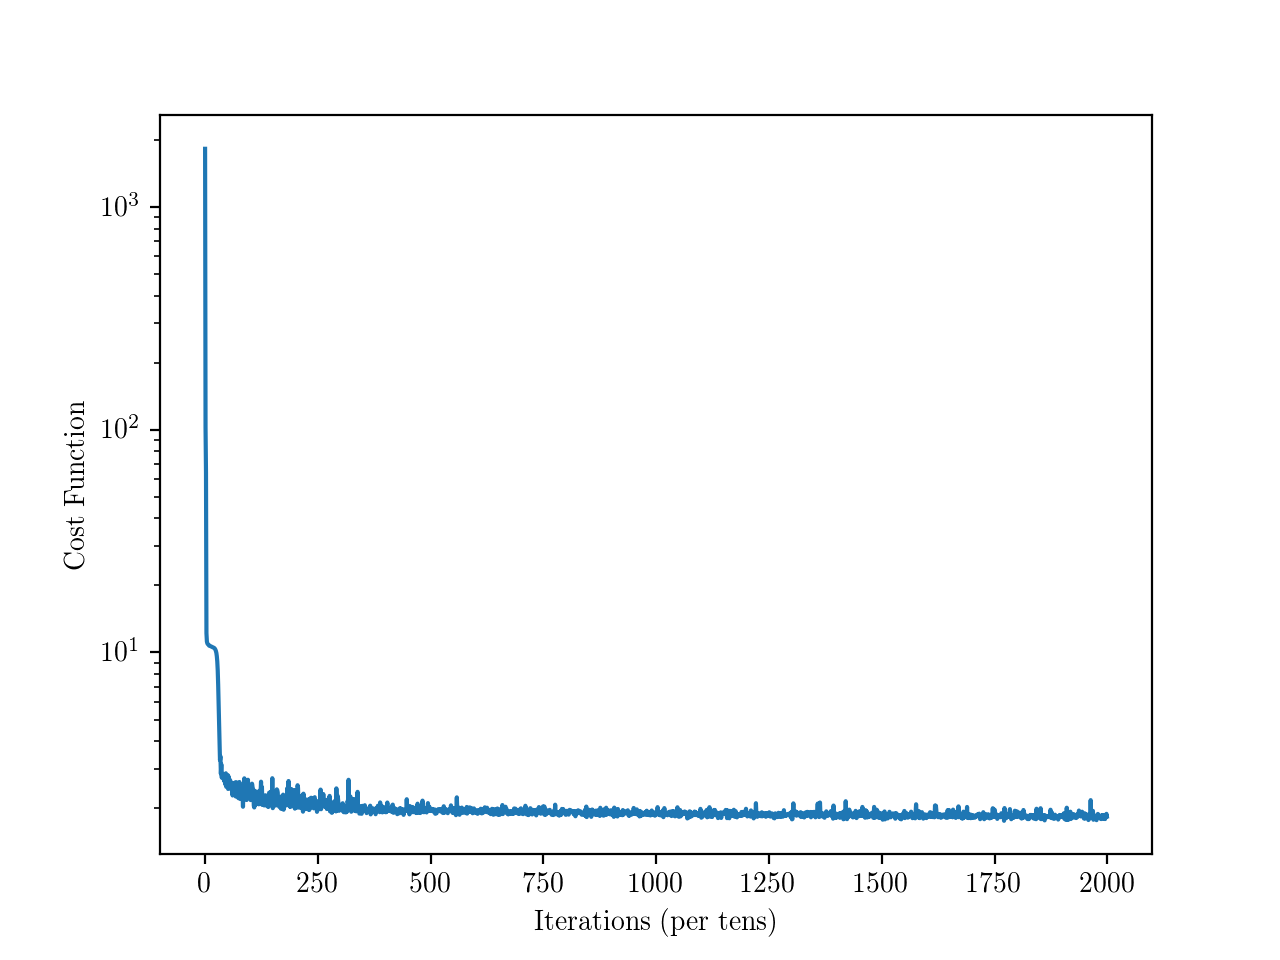
\includegraphics[scale=.5]{figures/final_cost_vs_epoch.png}
\caption{Cost versus epoch on the training data.}
\label{f-example_cost_vs_epoch}
\end{figure}

Figure~\ref{f-DFT_compare} is a plot comparing the real part of the DFT of an example in the test set 
versus its neural network estimate. The two graphs are very similar, but not identical; we 
find that for the particular example in Figure~\ref{f-DFT_compare}, 
$\|F\{f\} - \hat{F}\{f\}\|_2 / \|F\{f\}\|_2 = 6.0 \times 10^{-4}$. This result suggests that this particular
neural network architecutre for estimating the DFT of a vector is valid and can be used successfully.

\begin{figure}
\centering
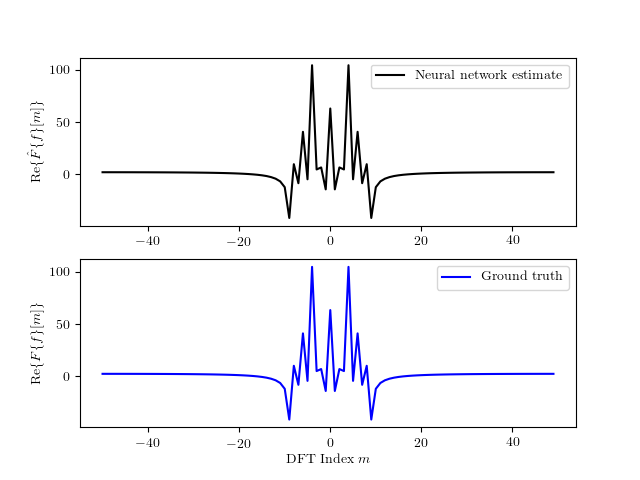
\includegraphics[scale=.65]{figures/DFT_comparisons.png}
\caption{The real part of the DFT of an example (bottom) and the estimate from the output of the neural network.}
\label{f-DFT_compare}
\end{figure}

\subsection{Timing}
Over the 3000 data examples in the test set, the naive implementation of the DFT averaged a time of 4.1 $\mu$s,
the FFT averaged a time of 3.5 $\mu$s, while our neural network implementation maintained a time of 1.9 $\mu$s, a time
faster than both the naive implementation and the FFT. These results show that there exists situations where the neural
network architecture is faster than the current state-of-the-art methods, at the cost of a negligible loss in accuracy.

\section{Future work}
% For the field of Fourier analysis with deep learning, there exists a multitude of unanswered questions that stem from 
% this research.

\paragraph{Exploiting structure.} It is well known that many signal processing problems become easier to solve if structure is
exploited, such as in compressed sensing, where sparsity is exploited to reduce the minimum sampling rate for perfect signal
reconstruction \cite{D:06}. It is possible that these efficients can further be explained or exploited using neural networks
with a potentially sparse amount of weights, compared to the neural network of a DFT.

\paragraph{Other transforms.} Although the DFT is the most widely known basis transformations, there exists a wide variety of
basis transforms that could be exploited using deep learning and with wide-ranging applications, such as the Discrete
Cosine transform in image compression \cite{ANR:74,YL:95}, the Radon transform in tomography \cite{D:07}, and the Continuous 
Wavelet transform \cite{M:08}. The creation of such a neural network would potentially allow for a much speedier implementation 
of a particular transform, designed for one particular task (\eg, image reconstruction from a fixed image size.)

\section{Contributions and acknowledgements}
This project was designed, written, and programmed by Jonathan Tuck. The code for this project can be viewed at 
\url{https://github.com/jonathantuck/CS230-project}.

The author would like to thank Xingyu Liu for his insightful comments on how to improve this project, and for suggesting 
neural network architectures to use for this particular application.

\newpage
\bibliography{template}

\end{document}

\end{document}